\chapter{Развертывание кластера}

\section{Конфигурирование узлов гипервизора}

\subsection{Первоначальная настройка управляющего узла}

Первым делом создадим управляющий узел кластера. Этот процесс отображен на рисунках \ref{init/01} -- \ref{init/10}

\begin{figure}[H]
	\centering
	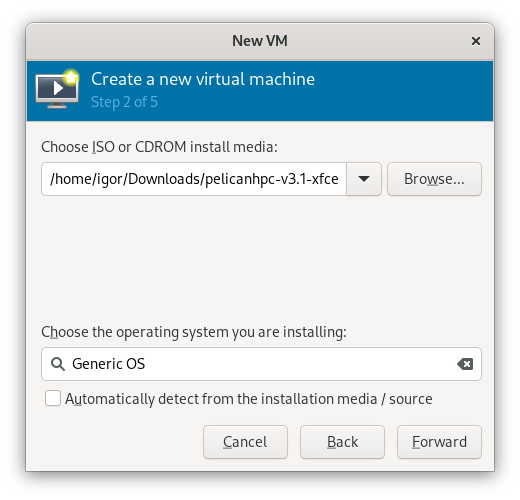
\includegraphics[width=0.5\linewidth]{1-01}
	\caption{Выбор образа ОС}
	\label{init/01}
\end{figure}

\begin{figure}[H]
	\centering
	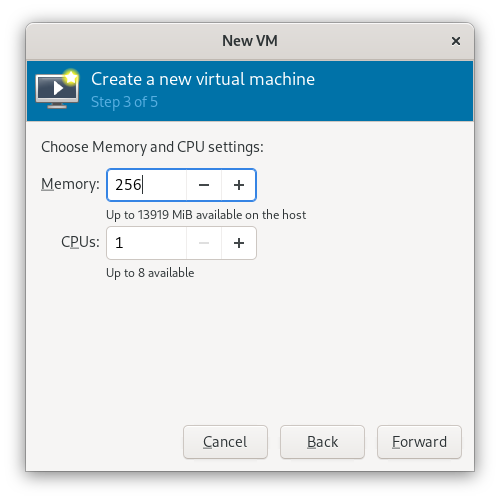
\includegraphics[width=0.5\linewidth]{1-02}
	\caption{Выделение ресурсов управляющему узлу}
	\label{init/02}
\end{figure}

\begin{figure}[H]
	\centering
	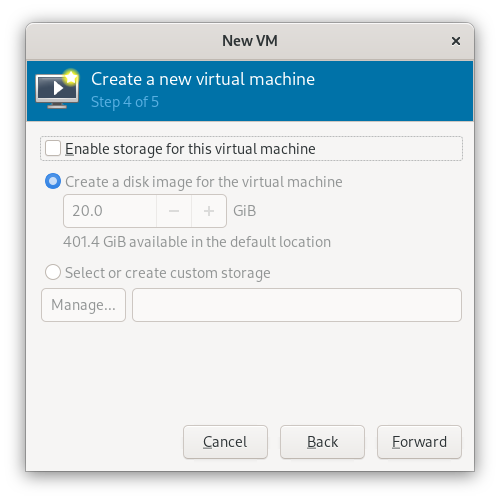
\includegraphics[width=0.5\linewidth]{1-03}
	\caption{Отключение дискового хранилища ВМ}
	\label{init/03}
\end{figure}

\begin{figure}[H]
	\centering
	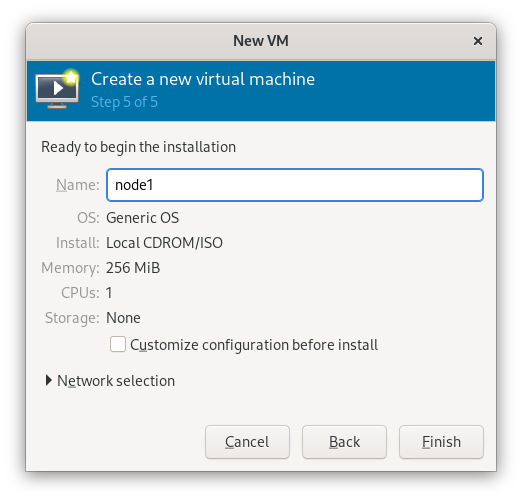
\includegraphics[width=0.5\linewidth]{1-04}
	\caption{Выбор имени ВМ}
	\label{init/04}
\end{figure}

\begin{figure}[H]
	\centering
	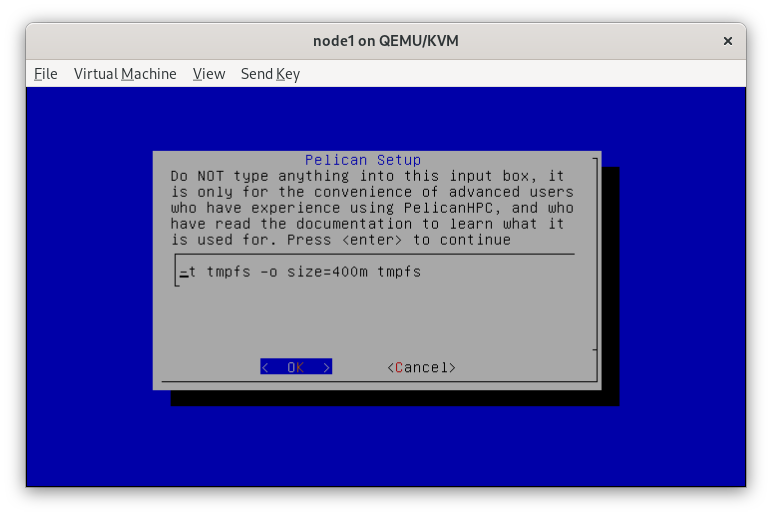
\includegraphics[width=0.7\linewidth]{1-05}
	\caption{Способ загрузки ОС}
	\label{init/05}
\end{figure}

\begin{figure}[H]
	\centering
	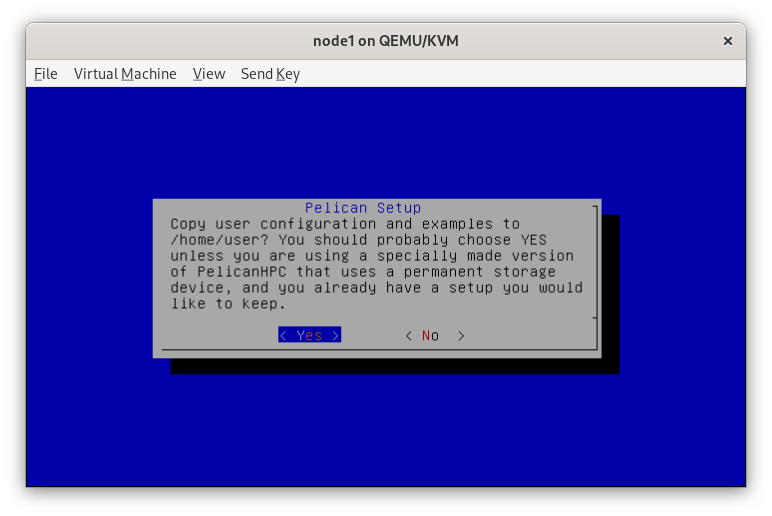
\includegraphics[width=0.7\linewidth]{1-06}
	\caption{Конфигурирование пользователя}
	\label{init/06}
\end{figure}

\begin{figure}[H]
	\centering
	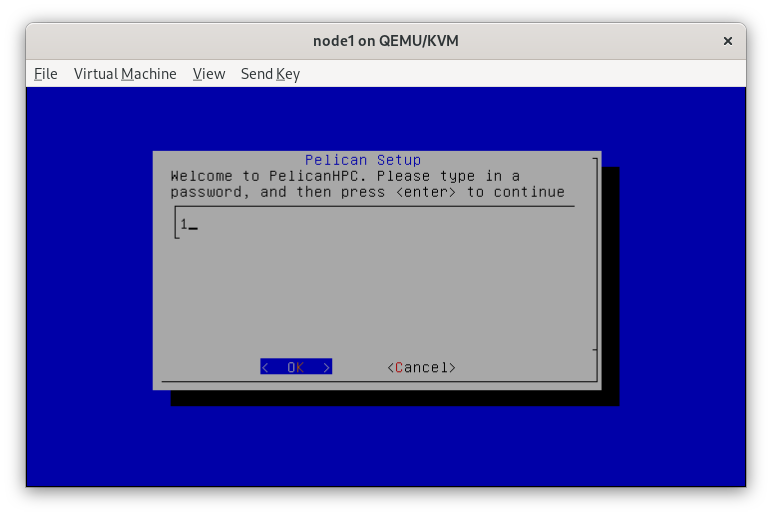
\includegraphics[width=0.7\linewidth]{1-07}
	\caption{Задание пароля пользователя}
	\label{init/07}
\end{figure}

\begin{figure}[H]
	\centering
	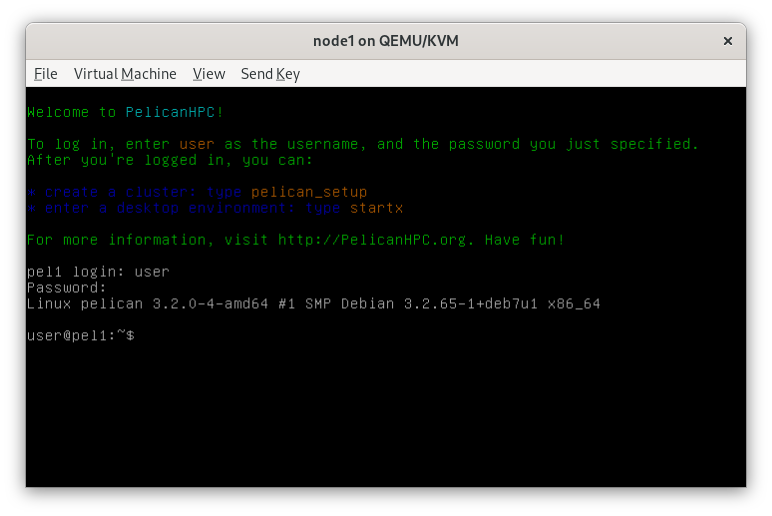
\includegraphics[width=0.7\linewidth]{1-08}
	\caption{Конфигурирование кластера}
	\label{init/08}
\end{figure}

\begin{figure}[H]
	\centering
	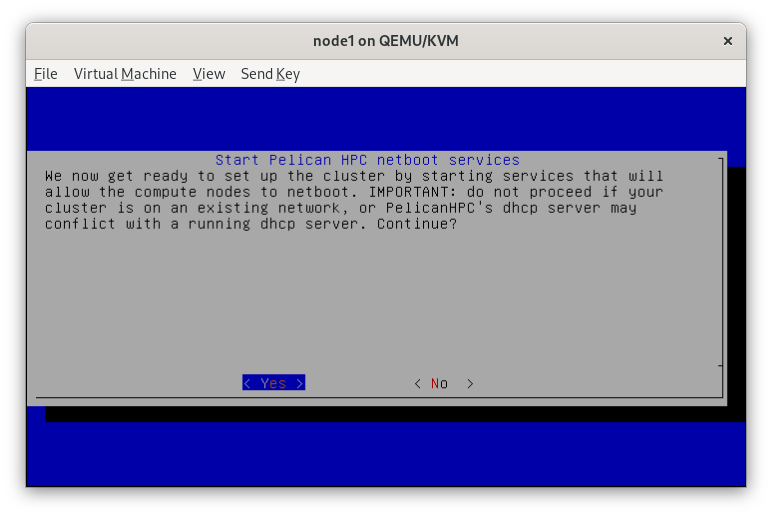
\includegraphics[width=0.7\linewidth]{1-09}
	\caption{Включение сетевого конфигурирование кластера}
	\label{init/09}
\end{figure}

\begin{figure}[H]
	\centering
	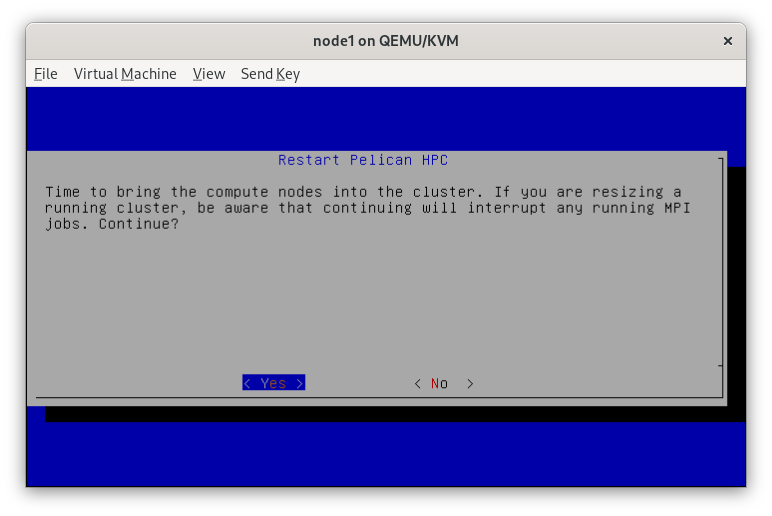
\includegraphics[width=0.7\linewidth]{1-10}
	\caption{Ожидание подключения узлов кластера}
	\label{init/10}
\end{figure}


\subsection{Включение узлов кластера}

Теперь необходимо развернуть узлы кластера. Основное требование к ним --- возможность загрузки ОС по сети. Скриншоты \ref{nodes/01} -- \ref{nodes/07} демострируют конфигурацию одного узла, однако все остальные узлы создаются с такими же параметрами.

\begin{figure}[H]
	\centering
	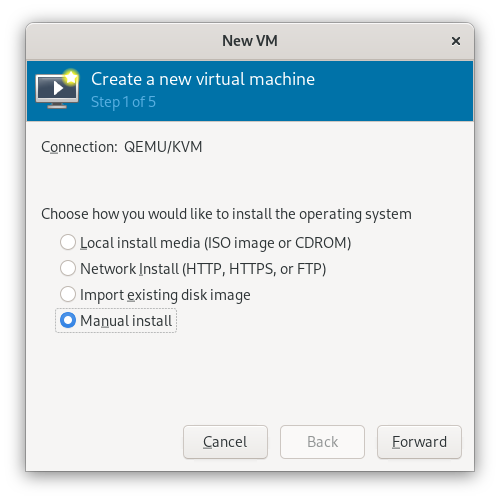
\includegraphics[width=0.5\linewidth]{2-01}
	\caption{Выбор способа установки}
	\label{nodes/01}
\end{figure}

\begin{figure}[H]
	\centering
	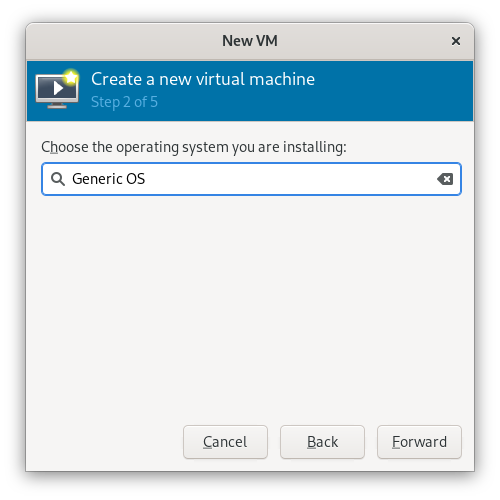
\includegraphics[width=0.5\linewidth]{2-02}
	\caption{Выбор типа образа}
	\label{nodes/02}
\end{figure}

\begin{figure}[H]
	\centering
	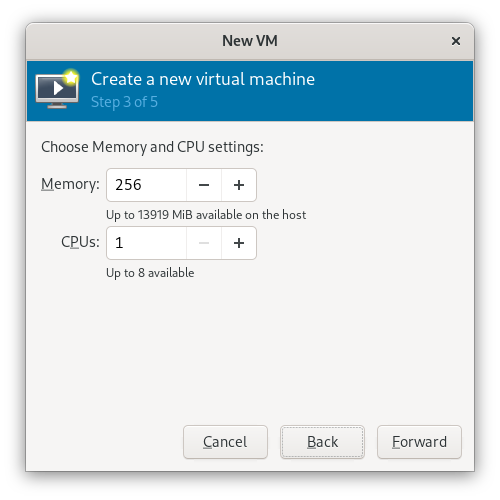
\includegraphics[width=0.5\linewidth]{2-03}
	\caption{Выделение ресурсов узлу}
	\label{nodes/03}
\end{figure}

\begin{figure}[H]
	\centering
	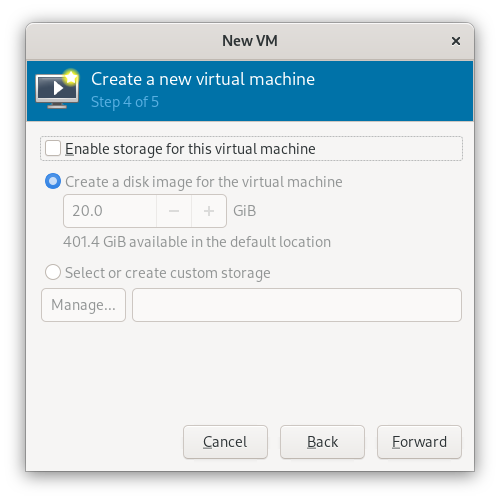
\includegraphics[width=0.5\linewidth]{2-04}
	\caption{Отключение дискового хранилища узла}
	\label{nodes/04}
\end{figure}

\begin{figure}[H]
	\centering
	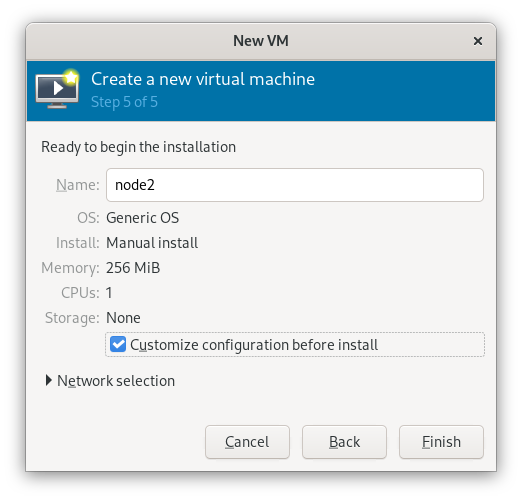
\includegraphics[width=0.5\linewidth]{2-05}
	\caption{Выбор имени узла}
	\label{nodes/05}
\end{figure}

\begin{figure}[H]
	\centering
	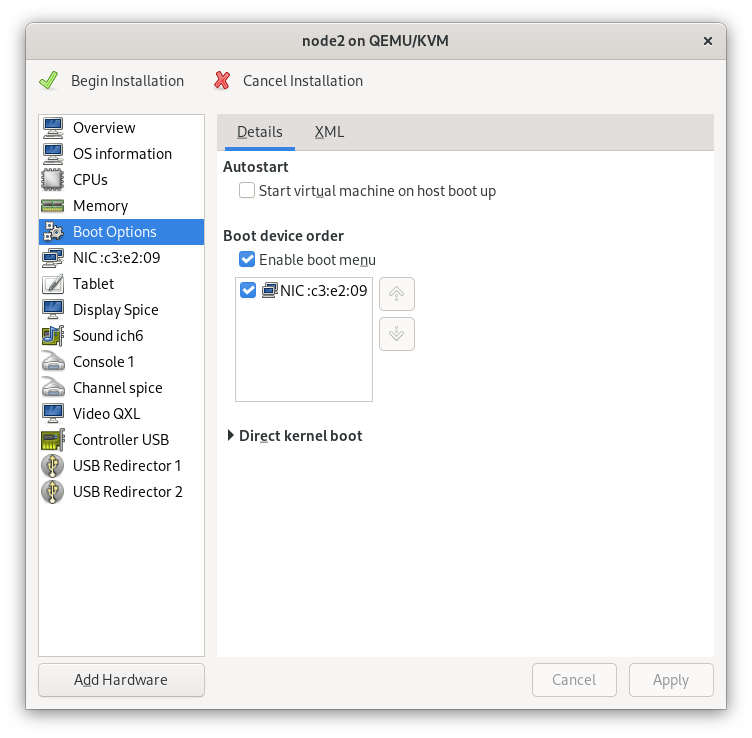
\includegraphics[width=0.7\linewidth]{2-06}
	\caption{Включение сетевой загрузки ОС}
	\label{nodes/06}
\end{figure}

\begin{figure}[H]
	\centering
	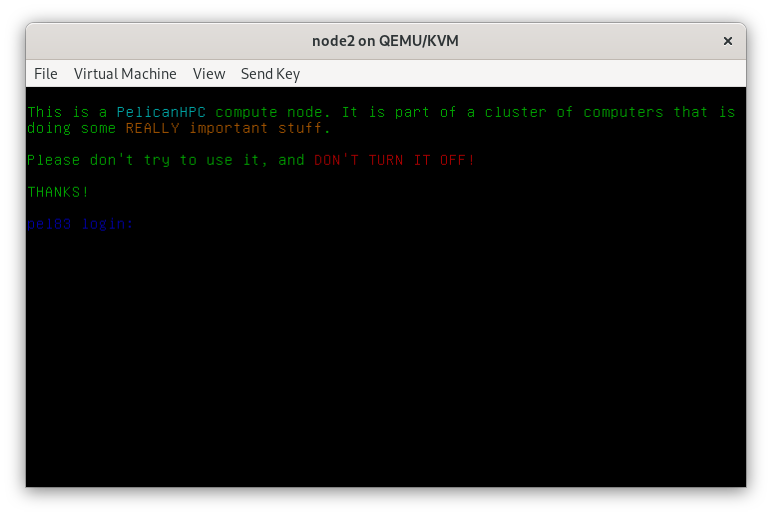
\includegraphics[width=0.7\linewidth]{2-07}
	\caption{Успешная загрузка узла}
	\label{nodes/07}
\end{figure}

\subsection{Донастройка кластера}

После успешного запуска всех узлов кластера нужно выполнить его донастройку. Рисунки \ref{postconf/01} -- \ref{postconf/03} демонстрируют этот процесс.

\begin{figure}[H]
	\centering
	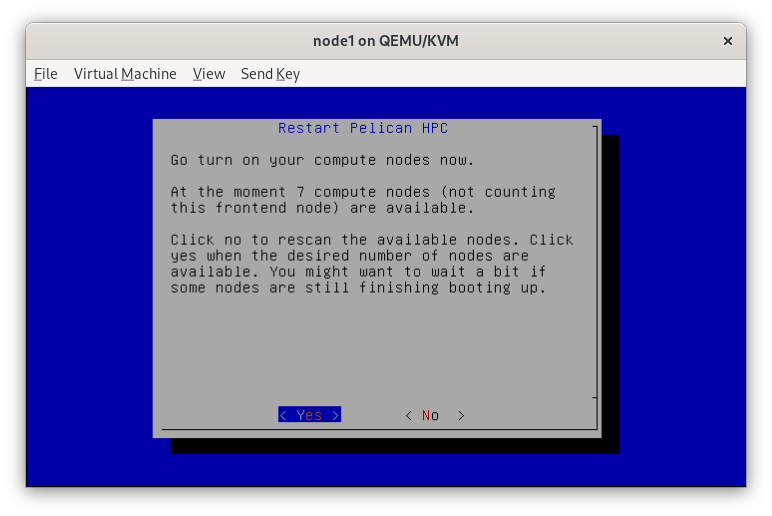
\includegraphics[width=0.7\linewidth]{3-01}
	\caption{Успешная загрузка узла}
	\label{postconf/01}
\end{figure}

\begin{figure}[H]
	\centering
	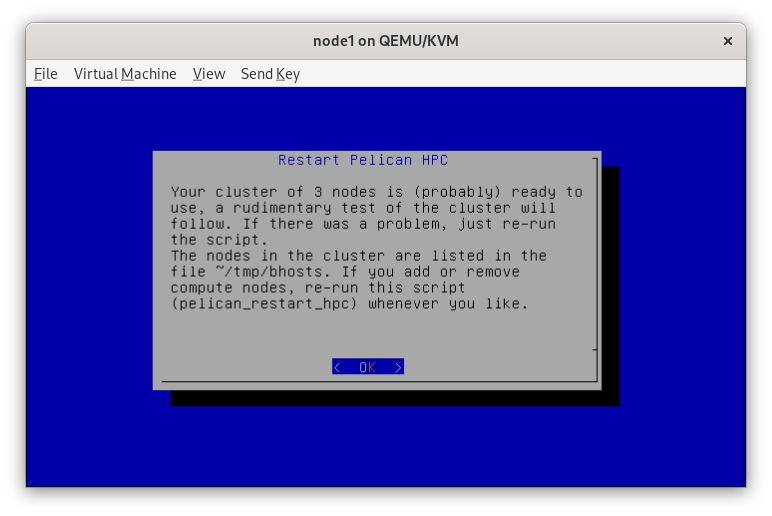
\includegraphics[width=0.7\linewidth]{3-02}
	\caption{Успешная загрузка узла}
	\label{postconf/02}
\end{figure}

\begin{figure}[H]
	\centering
	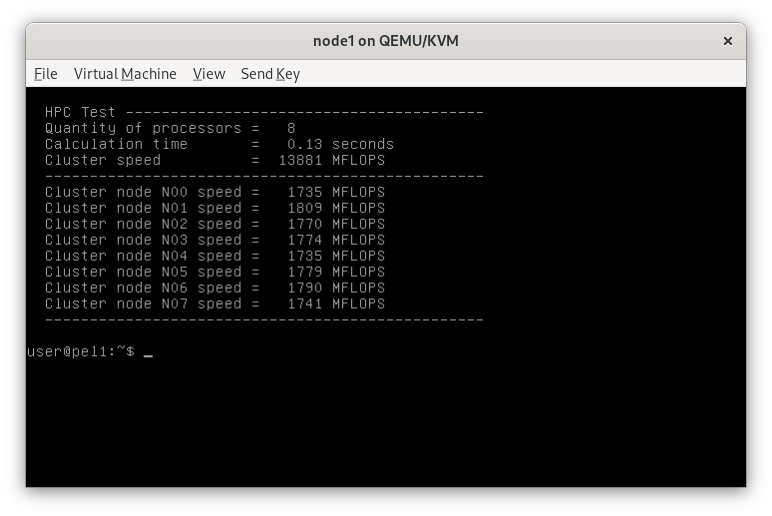
\includegraphics[width=0.7\linewidth]{3-03}
	\caption{Успешная загрузка узла}
	\label{postconf/03}
\end{figure}

\section{Тест кластера}
Выполним по 10 тестов для разного количества узлов кластера (1 - 8), чтобы получить усредненные значения. Результаты можно посмотреть в таблицах \ref{res/01} -- \ref{res/08}.

\begin{table}[H]
	\caption{Результаты для одного узла}
	\centering
	\begin{tabular}{|c|c|c|}
		\hline
\textbf{№ попытки} & \textbf{Время} & \textbf{MFLOPS} \\ \hline
		1  & 0.61 & 2933 \\ \hline
		2  & 0.61 & 2930 \\ \hline
		3  & 0.63 & 2848 \\ \hline
		4  & 0.63 & 2851 \\ \hline
		5  & 0.62 & 2911 \\ \hline
		6  & 0.62 & 2901 \\ \hline
		7  & 0.63 & 2871 \\ \hline
		8  & 0.61 & 2933 \\ \hline
		9  & 0.61 & 2946 \\ \hline
		10 & 0.62 & 2898 \\ \hline
\textbf{Среднее} & \textbf{0.62} & \textbf{2902} \\
		\hline
	\end{tabular}
	\label{res/01}
\end{table}


\begin{table}[H]
	\caption{Результаты для двух узлов}
	\centering
	\begin{tabular}{|c|c|c|}
		\hline
		\textbf{№ попытки} & \textbf{Время} & \textbf{MFLOPS} \\\hline
		1 & 0.33 & 5426 \\ \hline
		2 & 0.31 & 5807 \\ \hline
		3 & 0.34 & 5336 \\ \hline
		4 & 0.34 & 5228 \\ \hline
		5 & 0.33 & 5380 \\ \hline
		6 & 0.32 & 5545 \\ \hline
		7 & 0.33 & 5517 \\ \hline
		8 & 0.32 & 5553 \\ \hline
		9 & 0.32 & 5689 \\ \hline
		10 & 0.33 & 5453 \\ \hline
		\textbf{Среднее} & \textbf{0.33} & \textbf{5493} \\\hline
	\end{tabular}
	\label{res/02}
\end{table}


\begin{table}[H]
	\caption{Результаты для трех узлов}
	\centering
	\begin{tabular}{|c|c|c|}
		\hline
		\textbf{№ попытки} & \textbf{Время} & \textbf{MFLOPS} \\\hline
		1 & 0.22 & 8302 \\ \hline
		2 & 0.23 & 7746 \\ \hline
		3 & 0.24 & 7432 \\ \hline
		4 & 0.23 & 7826 \\ \hline
		5 & 0.28 & 6441 \\ \hline
		6 & 0.23 & 7873 \\ \hline
		7 & 0.23 & 7663 \\ \hline
		8 & 0.25 & 7311 \\ \hline
		9 & 0.25 & 7276 \\ \hline
		10 & 0.25 & 7329 \\ \hline
		\textbf{Среднее} & \textbf{0.24} & \textbf{7520} \\\hline
	\end{tabular}
	\label{res/03}
\end{table}


\begin{table}[H]
		\caption{Результаты для четырех узлов}
	\centering
	\begin{tabular}{|c|c|c|}
		\hline
		\textbf{№ попытки} & \textbf{Время} & \textbf{MFLOPS} \\\hline
		1 & 0.17 & 10508 \\ \hline
		2 & 0.18 & 10243 \\ \hline
		3 & 0.23 & 7966 \\ \hline
		4 & 0.18 & 10030 \\ \hline
		5 & 0.22 & 8211 \\ \hline
		6 & 0.18 & 10135 \\ \hline
		7 & 0.21 & 8552 \\ \hline
		8 & 0.21 & 8721 \\ \hline
		9 & 0.18 & 10153 \\ \hline
		10 & 0.18 & 10252 \\ \hline
		\textbf{Среднее} & \textbf{0.19} & \textbf{9477} \\\hline
	\end{tabular}
	\label{res/04}
\end{table}


\begin{table}[H]
	\caption{Результаты для пяти узлов}
	\centering
	\begin{tabular}{|c|c|c|}
		\hline
		\textbf{№ попытки} & \textbf{Время} & \textbf{MFLOPS} \\\hline
		1 & 0.18 & 9762 \\ \hline
		2 & 0.18 & 9887 \\ \hline
		3 & 0.19 & 9608 \\ \hline
		4 & 0.19 & 9626 \\ \hline
		5 & 0.19 & 9307 \\ \hline
		6 & 0.19 & 9677 \\ \hline
		7 & 0.19 & 9311 \\ \hline
		8 & 0.22 & 8126 \\ \hline
		9 & 0.18 & 10204 \\ \hline
		10 & 0.19 & 9698 \\ \hline
		\textbf{Среднее} & \textbf{0.19} & \textbf{9521} \\\hline
	\end{tabular}
	\label{res/05}
\end{table}


\begin{table}[H]
	\caption{Результаты для шести узлов}
	\centering
	\begin{tabular}{|c|c|c|}
		\hline
		\textbf{№ попытки} & \textbf{Время} & \textbf{MFLOPS} \\\hline
		1 & 0.16 & 11064 \\ \hline
		2 & 0.16 & 11153 \\ \hline
		3 & 0.19 & 9350 \\ \hline
		4 & 0.19 & 9322 \\ \hline
		5 & 0.16 & 11101 \\ \hline
		6 & 0.16 & 11125 \\ \hline
		7 & 0.20 & 9197 \\ \hline
		8 & 0.16 & 11047 \\ \hline
		9 & 0.16 & 11079 \\ \hline
		10 & 0.18 & 10251 \\ \hline
		\textbf{Среднее} & \textbf{0.19} & \textbf{10469} \\\hline
	\end{tabular}
	\label{res/06}
\end{table}


\begin{table}[H]
	\caption{Результаты для семи узлов}
	\centering
	\begin{tabular}{|c|c|c|}
		\hline
		\textbf{№ попытки} & \textbf{Время} & \textbf{MFLOPS} \\\hline
		1 & 0.14 & 12537 \\ \hline
		2 & 0.14 & 12730 \\ \hline
		3 & 0.17 & 10530 \\ \hline
		4 & 0.17 & 10361 \\ \hline
		5 & 0.14 & 12682 \\ \hline
		6 & 0.14 & 12430 \\ \hline
		7 & 0.17 & 10609 \\ \hline
		8 & 0.17 & 10657 \\ \hline
		9 & 0.14 & 12693 \\ \hline
		10 & 0.14 & 12630 \\ \hline
		\textbf{Среднее} & \textbf{0.15} & \textbf{11786} \\\hline
	\end{tabular}
	\label{res/07}
\end{table}


\begin{table}[H]
	\caption{Результаты для восьми узлов}
	\centering
	\begin{tabular}{|c|c|c|}
		\hline
		\textbf{№ попытки} & \textbf{Время} & \textbf{MFLOPS} \\\hline
		1 & 0.13 & 13650 \\ \hline
		2 & 0.13 & 14070 \\ \hline
		3 & 0.16 & 11504 \\ \hline
		4 & 0.13 & 13853 \\ \hline
		5 & 0.13 & 13456 \\ \hline
		6 & 0.13 & 13820 \\ \hline
		7 & 0.16 & 11101 \\ \hline
		8 & 0.13 & 13826 \\ \hline
		9 & 0.13 & 13799 \\ \hline
		10 & 0.13 & 13789 \\ \hline
		\textbf{Среднее} & \textbf{0.14} & \textbf{13290} \\\hline
	\end{tabular}
	\label{res/08}
\end{table}


Визуализируем полученные результаты в виде графиков. Они продемострированы на рисунках \ref{plot/01} и \ref{plot/02}.


\begin{figure}[H]
	\centering
	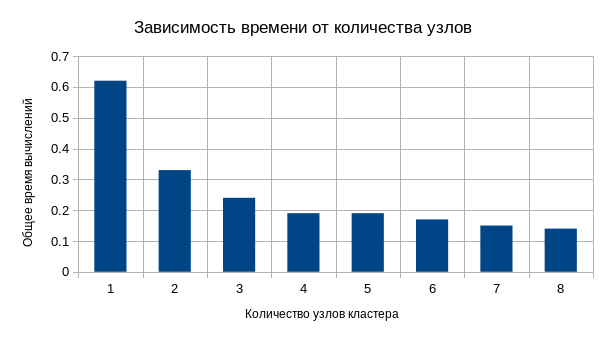
\includegraphics[width=\linewidth]{4-01}
	\caption{График времени}
	\label{plot/01}
\end{figure}


\begin{figure}[H]
	\centering
	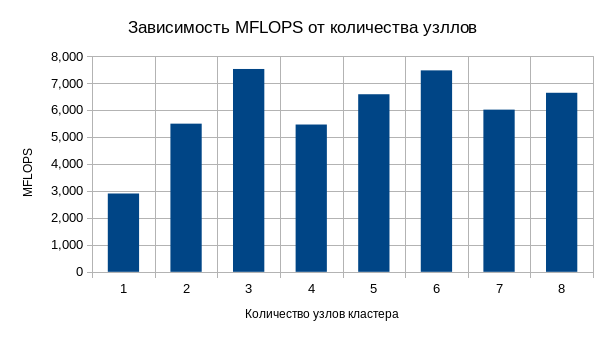
\includegraphics[width=\linewidth]{4-02}
	\caption{График MFLOPS}
	\label{plot/02}
\end{figure}


\section{Анализ полученных результатов}

Если смотреть на графики \ref{plot/01} и \ref{plot/02}, то можно заметить, что с увеличением количества вычислительных узлов в два раза, время и MFLOPS сокращаются/увеличиваются соответственно в два раза только на первом шаге, затем различия становятся все менее значимыми. Это можно объяснить суммой задержек (траспортной и синхронизации) и особенностью тестовой задачи. Вполне вероятно, что другая задача может выдать другие результаты, которые окажутся хуже или лучше полученных.

Анализ таблиц \ref{res/01} -- \ref{res/08} показывается, что с ростом количества узлов выростоет стабильность (или уменьшатся разброс показателей времени и MFLOPS).
